% Softmax Numerics and Attention Sinks in LLM Serving: a reproduction and measurement study
% TMLR style (JmlrOrg/tmlr-style-file @7bf90ef), preprint option. Build: make pdf  (or latexmk -pdf main.tex)
% Every number comes from generated/macros.tex or generated/tab_*.tex, written by gen_latex.py from ../data.
\documentclass[10pt]{article}
\usepackage[preprint]{tmlr}
\usepackage[utf8]{inputenc}
\usepackage[T1]{fontenc}
\usepackage{lmodern}
\usepackage{amsmath,amssymb}
\usepackage{booktabs}
\usepackage{graphicx}
\usepackage{xcolor}
\usepackage{enumitem}
\usepackage{hyperref}
\usepackage{url}
\usepackage[switch]{lineno}
\hypersetup{colorlinks=true,linkcolor=blue!60!black,citecolor=blue!60!black,urlcolor=blue!60!black,
  pdftitle={Softmax Numerics and Attention Sinks in LLM Serving},pdfauthor={Tata Vishnu Vardhan Rao}}
% generated by gen_latex.py from ../data; do not edit
\newcommand{\cliffBfTwo}{5.547}
\newcommand{\cliffFpTwo}{16.636}
\newcommand{\cliffBfMany}{5.564}
\newcommand{\cliffFpMany}{15.943}
\newcommand{\cliffHalfMany}{7.622}
\newcommand{\cliffDblTwo}{36.737}
\newcommand{\cliffDblMany}{34.658}
\newcommand{\cliffDblEarly}{2.08}
\newcommand{\cliffFpEarly}{0.69}
\newcommand{\fixHalfZeroGap}{17.336}
\newcommand{\fixRelErrFp}{$3.2\times10^{-7}$}
\newcommand{\fixRelErrBf}{$9.7\times10^{-3}$}
\newcommand{\cancFloorFp}{$9.14\times10^{-9}$}
\newcommand{\cancFloorBf}{$1.22\times10^{-3}$}
\newcommand{\cancFloorHalf}{$2.27\times10^{-4}$}
\newcommand{\cancDecompStudent}{$1.08\times10^{-3}$}
\newcommand{\cancDecompTeacher}{$3.29\times10^{-4}$}
\newcommand{\cancMixedBf}{$2.2\times10^{-8}$}
\newcommand{\polyLo}{0.849}
\newcommand{\polyHi}{5.945}
\newcommand{\polyBetaMax}{2.42}
\newcommand{\logpBfGap}{17.44}
\newcommand{\logpFpGap}{27.88}
\newcommand{\pplQwen}{31.6}
\newcommand{\pplGemma}{39.9}
\newcommand{\pplSmol}{17.0}
\newcommand{\pplVanilla}{17.3}
\newcommand{\sinkFirstVanilla}{62.6}
\newcommand{\sinkLastVanilla}{10.6}
\newcommand{\sinkLastNVanilla}{4,096}
\newcommand{\needleFixedFirstVanilla}{0.782}
\newcommand{\needleFixedLastVanilla}{0.0019}
\newcommand{\needleBestLastVanilla}{0.767}
\newcommand{\needleTopOneVanilla}{15/15}
\newcommand{\pplSoftpick}{17.1}
\newcommand{\sinkFirstSoftpick}{0.0}
\newcommand{\sinkLastSoftpick}{0.0}
\newcommand{\sinkLastNSoftpick}{4,096}
\newcommand{\needleFixedFirstSoftpick}{0.690}
\newcommand{\needleFixedLastSoftpick}{0.0737}
\newcommand{\needleBestLastSoftpick}{0.635}
\newcommand{\needleTopOneSoftpick}{14/15}

\newcommand{\pending}[1]{\textcolor{orange!70!black}{\textbf{[Pending:} #1\textbf{]}}}
\newif\ifdraft\drafttrue
\ifdraft\linenumbers\fi

\title{Softmax Numerics and Attention Sinks in LLM Serving:\\ A Reproduction and Measurement Study}
\author{\name Tata Vishnu Vardhan Rao \email tatavishnurao@gmail.com\\
  \addr Anurag University, Hyderabad, India}
\def\month{11}\def\year{2026}\def\openreview{}

\begin{document}
\maketitle

\begin{abstract}
Serving engines compute softmax in every attention head and in the vocabulary head. We re-test four published claims about it: dispersion with growing context and an adaptive-temperature fix, first-token attention sinks, Softmax Collapse, and Softmax Cancellation. We use fine-grid CPU reproductions and the papers' own published code. The published collapse cliffs (5.5, 16.6, 36.7 nats) are two-class values: with $\geq$113 classes, CPU PyTorch collapses up to \cliffDblEarly{} nats earlier. The published adaptive-temperature polynomial acts only on rows with entropy between \polyLo{} and \polyHi{} nats. In a matched 340M softmax/softpick pair, the softmax model's sink rate falls from \sinkFirstVanilla\% to \sinkLastVanilla\% between 256 and 4,096 tokens, while softpick shows none. We also locate where vLLM and SGLang compute returned log-probabilities; SGLang's RL on-policy mode uses bfloat16. Code, data and validation logs are released.
\end{abstract}

\ifdraft
\noindent\fbox{\parbox{\dimexpr\linewidth-2\fboxsep}{\small\textbf{Working draft, \today.} Real-model results cover the models whose runs have finished; the others, E7 on real text and the GPU experiments (B4--B6) are marked \pending{\dots}. Set \texttt{\textbackslash draftfalse} to remove line numbers and this box.}}
\fi

\section{Introduction}
A served language model evaluates softmax in every attention head and again in the vocabulary head. Four recent claims about it matter for serving:
\begin{itemize}[leftmargin=*,itemsep=1pt]
\item global attention must disperse as context grows, and an entropy-based adaptive temperature partly counters this \citep{velickovic};
\item the first-token attention sink is a learned mechanism that limits over-mixing \citep{barbero};
\item standard cross-entropy has a precision cliff beyond which the target gradient is exactly zero, \emph{Softmax Collapse} \citep{prieto,barron};
\item soft-target cross-entropy leaves a non-zero gradient when student and teacher agree, \emph{Softmax Cancellation} \citep{barron}.
\end{itemize}
Serving engines inherit these behaviours. Eviction policies decide which keys to keep \citep{streamingllm}, kernels fold learned sinks into the normaliser \citep{flashattn}, and RL trainers consume returned log-probabilities \citep{sglang}.

This paper re-tests the four claims and measures the related behaviour in five open models. It proposes no new method. Following the reproducibility-report format of TMLR and the ML Reproducibility Challenge \citep{lico}, each claim is stated with its source, tested, and given a verdict. Following measurement papers on LLM serving \citep{etalon,measbias}, we report where a standard computation returns a misleading number. Our contributions:
\begin{enumerate}[leftmargin=*,itemsep=1pt]
\item a reproduction of four claims on CPU PyTorch, with fine grids, float64 and 50-digit references, and the papers' published code translated line by line (\S\ref{sec:repro});
\item real-model measurements of sink strength and planted-needle retrieval in five open models, including a matched softmax/softpick pair \citep{softpickckpt}, with every probe validated bit for bit against the reference attention (\S\ref{sec:real});
\item an audit of how vLLM and SGLang compute returned log-probabilities (\S\ref{sec:logprob});
\item scripts for the remaining GPU experiments, one of them with a pre-registered success criterion (\S\ref{sec:artifact}).
\end{enumerate}

\section{Claims checked}
\begin{table}[t]
\centering\small
\caption{Claims, sources and verdicts (details in \S\ref{sec:repro}--\ref{sec:real}).}\label{tab:claims}
\begin{tabular}{p{0.6cm}p{5.6cm}p{2.6cm}p{4.4cm}}
\toprule
\# & Claim (paraphrased) & Source & Verdict \\
\midrule
C1a & With bounded logits, every global-attention coefficient is $\Theta(1/n)$ & \citet[Thm.~2.2]{velickovic} & Fixed heads disperse; other heads take over (3 of 5 models run) \\
C1b & Entropy-based adaptive temperature sharpens attention at inference & \citet[Fig.~4]{velickovic} & Holds inside the fitted regime; inactive above \polyHi{} nats \\
C2 & First-token sinks are common; non-normalised attention removes them & \citet{barbero,gu,softpick} & Holds in the matched pair \\
C3 & Target gradient is zero beyond $c\approx5.5$ (bf16), 16.6 (fp32), 36.7 (fp64) & \citet[\S1--2]{barron} & Holds for $C{=}2$; earlier for $C\geq113$ \\
C4 & Non-zero gradient at $z_S{=}z_T$; the fix returns 0 & \citet[\S3]{barron} & Holds \\
\bottomrule
\end{tabular}
\end{table}

\section{Methodology}
\paragraph{Synthetic reproductions.} All of these ran on CPU PyTorch 2.15.0, so every threshold below is a property of CPU kernels.
\begin{itemize}[leftmargin=*,itemsep=1pt]
\item \textbf{C3:} $C$ classes, target logit at gap $g$ above all others, built-in \texttt{F.cross\_entropy}. We scan $g$ on a 0.01 grid refined to 0.001 near each transition, and report the paper's margin $m=z_t-\mathrm{LSE}_{j\neq t}z_j=g-\ln(C-1)$.
\item \textbf{C4:} 1,000 classes. The reference is float64 $q-p$ on the same rounded logits, checked against mpmath at 50 digits.
\item \textbf{The fixes} are line-by-line translations of the paper's JAX listings.
\end{itemize}

\paragraph{Real-model probes.} Five models run in float32 on CPU (Table~\ref{tab:models}). We register an attention function with the transformers attention interface. It computes exact softmax (or softpick) attention in query chunks and records statistics as it runs.
\begin{itemize}[leftmargin=*,itemsep=1pt]
\item \textbf{Validation:} logits match transformers' eager attention bit for bit for all five models. For the matched pair they also match an independent forward pass written from the authors' code.
\item \textbf{Sensitivity:} swapping softpick for softmax in that reference changes the logits by up to 30.9, so the check does detect errors.
\item \textbf{Loading:} perplexity on 1,024 held-out tokens is 17--40 for all five models.
\end{itemize}

\begin{table}[t]
\centering\small
\caption{Models probed. Perplexity on 1,024 tokens of Project Gutenberg \#84, eager attention.}\label{tab:models}
\begin{tabular}{llllr}
\toprule
Model & Layers $\times$ heads & Attention & Context probed & PPL \\
\midrule
Qwen3-0.6B & $28\times16$ (8 KV) & global, QK-norm & 256--8,192 & \pplQwen \\
Gemma-3-1B-it & $26\times4$ (1 KV) & 5 local (512) : 1 global & 256--8,192 & \pplGemma \\
SmolLM2-360M & $32\times15$ (5 KV) & global & 256--8,192 & \pplSmol \\
vanilla-340M & $24\times16$ & global, softmax & 256--4,096 & \pplVanilla \\
softpick-340M & $24\times16$ & global, softpick & 256--4,096 & \pplSoftpick \\
\bottomrule
\end{tabular}
\end{table}

\paragraph{Metrics.} Probe statistics use the last 64 query positions of each sequence.
\begin{itemize}[leftmargin=*,itemsep=1pt]
\item \textbf{Sink rate:} the share of heads whose mean weight on token~0 exceeds 0.3 \citep{gu}.
\item \textbf{Needle weight:} the final query's weight on a planted sentence's answer tokens. We report it for the best head at each $N$, and for a fixed head (the best head at $N{=}256$). Under the fixed-gap law $w=e^{\Delta}/(e^{\Delta}+N-1)$, the fitted gap $\Delta_N=\mathrm{logit}(w)+\ln(N-1)$ stays constant.
\item \textbf{Sampling:} three Gutenberg passages and three needle depths per point.
\end{itemize}

\section{Reproduction results}\label{sec:repro}
\subsection{C3: Softmax Collapse}
\begin{table}[h]
\centering\small
\caption{Precision cliff in the paper's margin units: published value vs.\ first exact zero on CPU PyTorch.}\label{tab:cliffs}
\begin{tabular}{lrrrrr}
\toprule
dtype & published & $C{=}2$ & $C{=}113$ & $C{=}1000$ & $C{=}151{,}936$ \\
\midrule
bfloat16 & $\approx$5.5 & 5.547 & 5.564 & 5.562 & 5.507 \\
float16 & -- & 7.624 & 7.622 & 7.621 & 7.593 \\
float32 & $\approx$16.6 & 16.636 & 15.943 & 15.944 & 15.943 \\
float64 & $\approx$36.7 & 36.737 & 34.658 & 34.659 & 34.658 \\
\bottomrule
\end{tabular}

\end{table}
\begin{figure}[t]
\centering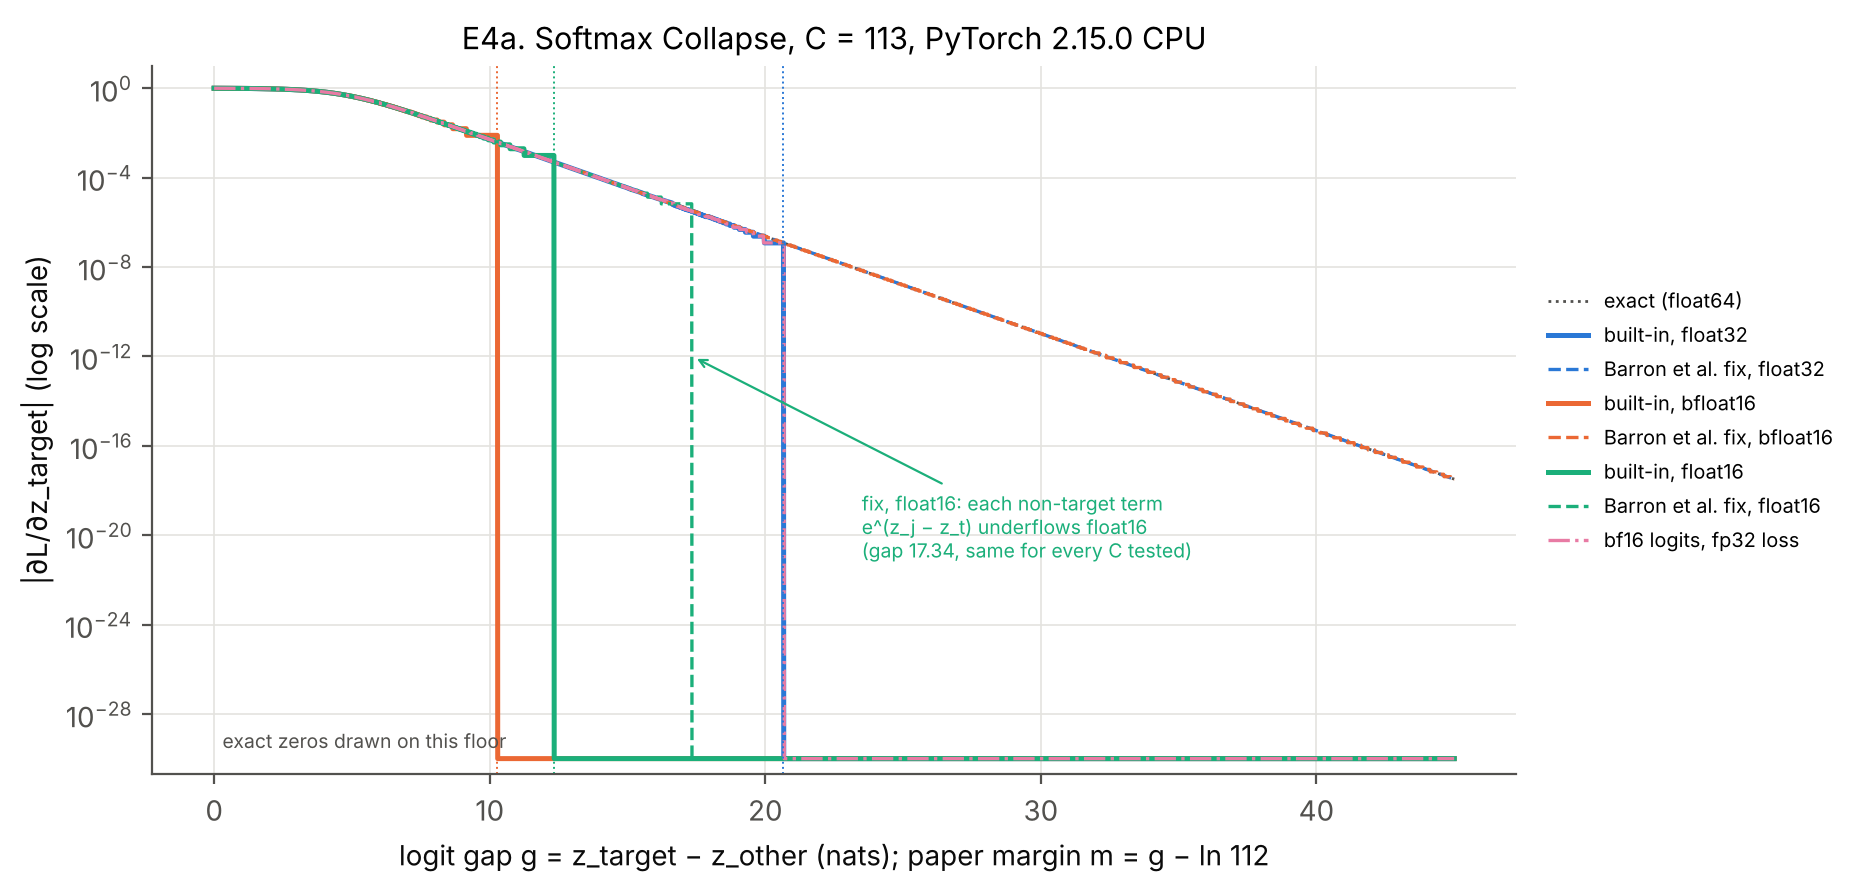
\includegraphics[width=0.92\linewidth]{figures/e4_collapse.png}
\caption{Target-logit gradient vs.\ logit gap, $C{=}113$, CPU PyTorch 2.15.0. Solid lines are built-in; dashed lines are the translated fix; dash-dot is bf16 logits with an fp32 loss. Exact zeros are drawn on the floor.}\label{fig:collapse}
\end{figure}
\textbf{Verdict: holds, with a class-count condition} (Table~\ref{tab:cliffs}, Figure~\ref{fig:collapse}).
\begin{itemize}[leftmargin=*,itemsep=1pt]
\item The published cliffs are the two-class values $\ln(2/\epsilon)$.
\item With $\geq113$ classes, CPU PyTorch collapses earlier: by \cliffFpEarly{} nats in fp32 and \cliffDblEarly{} nats in fp64. bf16 and fp16 stay within 0.04 of $\ln(2/\epsilon)$.
\item The fix never returns a zero target gradient in fp32 or bf16 (maximum relative error \fixRelErrFp{} and \fixRelErrBf). In fp16 it returns zero from gap \fixHalfZeroGap{} for every $C$ tested, because each $e^{z_j-z_t}$ underflows there.
\item With bf16 logits and an fp32 loss, the bf16 cliff disappears and the fp32 cliff remains.
\end{itemize}

\subsection{C4: Softmax Cancellation}
\textbf{Verdict: holds.} At $z_S=z_T$ the built-in gradient norm is \cancFloorFp{} (fp32), \cancFloorBf{} (bf16) and \cancFloorHalf{} (fp16); the fix returns exactly 0. Two storage choices drive the bf16 floor: the student's log-softmax stored in bf16 contributes \cancDecompStudent, and the teacher's probabilities stored in bf16 contribute \cancDecompTeacher. With fp32 teacher probabilities and an upcast student, the floor is \cancMixedBf.

\subsection{C1b: Adaptive temperature}
\begin{figure}[t]
\centering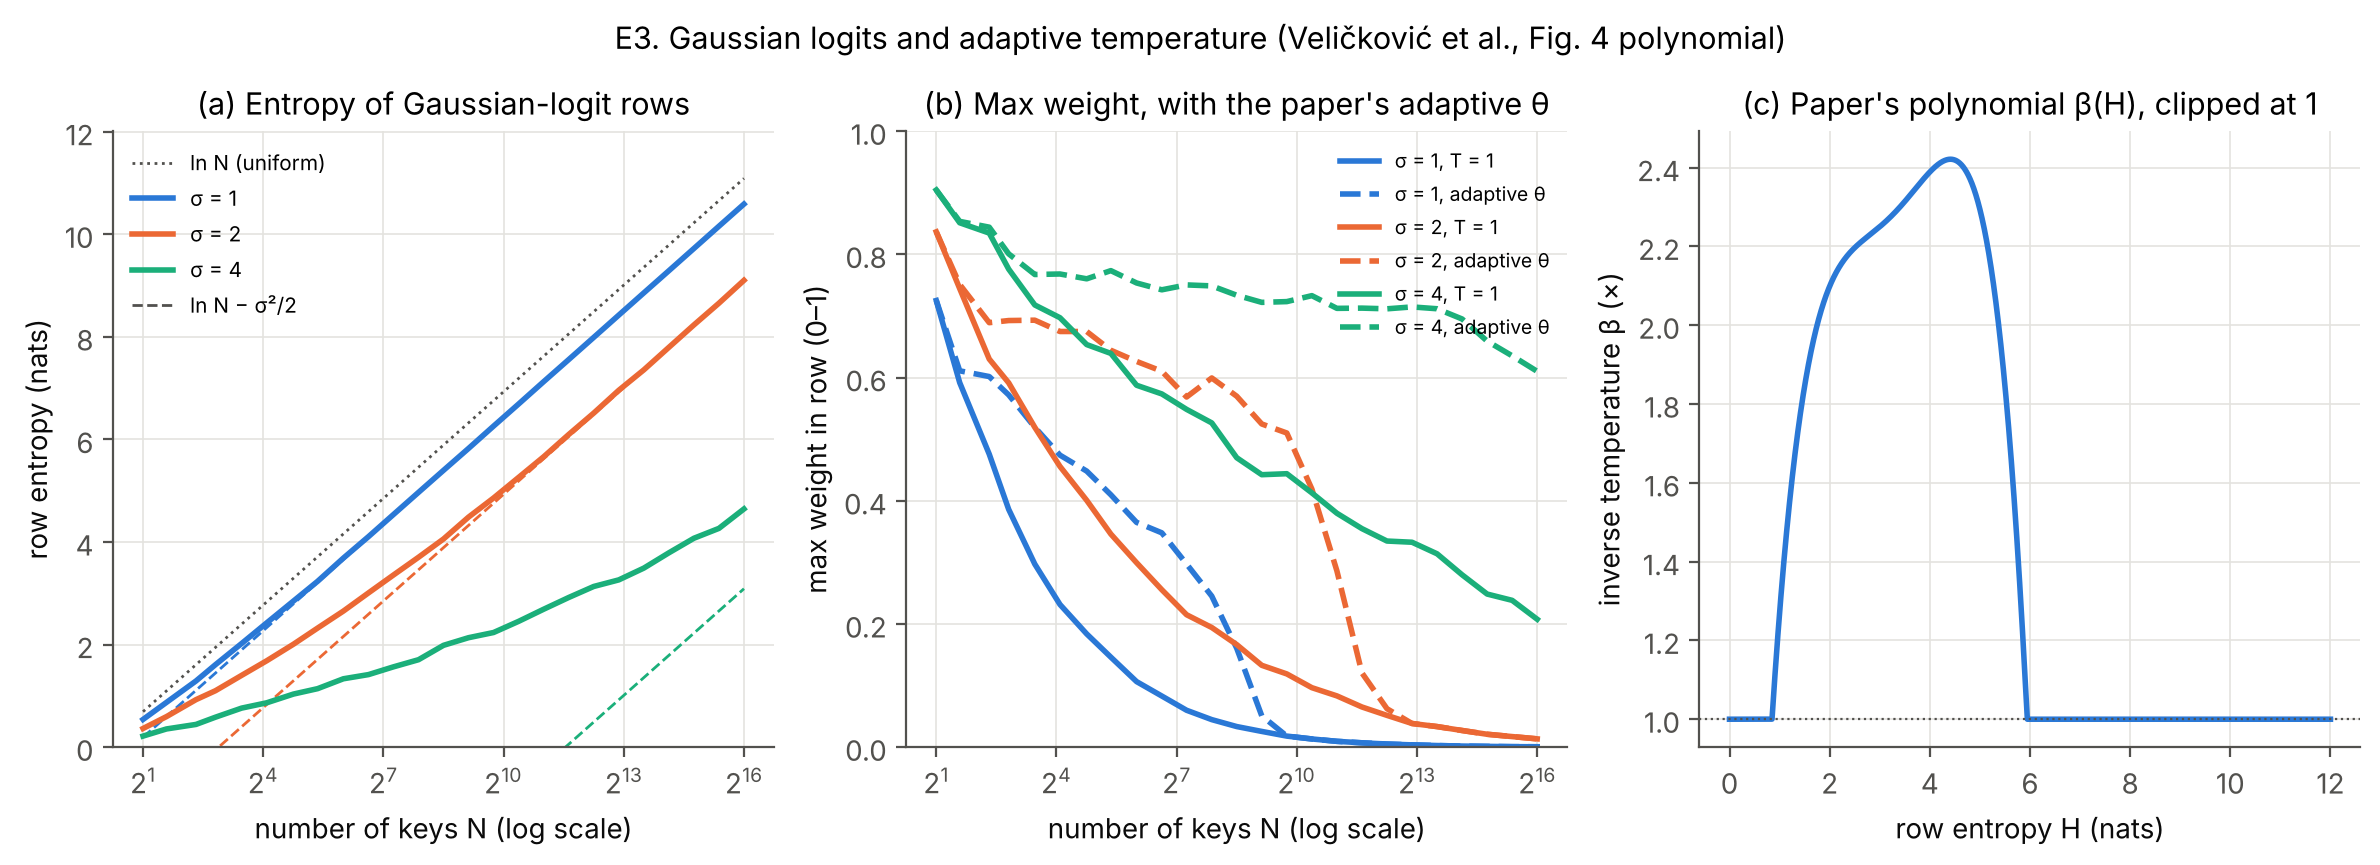
\includegraphics[width=\linewidth]{figures/e3_random_logits.png}
\caption{Gaussian-logit rows: entropy, maximum weight with and without the paper's adaptive $\theta$, and the polynomial $\beta(H)$ clipped at 1.}\label{fig:adaptive}
\end{figure}
\textbf{Verdict: holds inside the fitted regime; inactive beyond it} (Figure~\ref{fig:adaptive}).
\begin{itemize}[leftmargin=*,itemsep=1pt]
\item The printed polynomial gives $\beta>1$ only for $H\in[\polyLo,\polyHi]$ nats, peaking at $\beta=\polyBetaMax$.
\item A target planted $4\sigma$ above Gaussian distractors rises from 0.125 to 0.798 of the row at $N=235$.
\item The correction switches off from $N=861$. A uniform row over 4,096 keys already has 8.3 nats, so the fit needs refitting before use on long-context heads, as the authors' own description of it as ad hoc suggests \citep{velickovic}.
\end{itemize}

\section{Real-model measurements}\label{sec:real}
\begin{table}[t]
\centering\small
\caption{Sinks and planted-needle retrieval (last 64 queries; 3 passages and 3 needle depths per length).}\label{tab:e6}
\resizebox{\linewidth}{!}{\begin{tabular}{lrrrrrl}
\toprule
model & $N_{\max}$ & sink rate (256) & sink rate ($N_{\max}$) & fixed-head $w$ (256$\to N_{\max}$) & best-head $w$ ($N_{\max}$) & top-1 \\
\midrule
Qwen3-0.6B & \multicolumn{6}{l}{\emph{pending}} \\
Gemma-3-1B-it & \multicolumn{6}{l}{\emph{pending}} \\
SmolLM2-360M & 8,192 & 73.3\% & 41.0\% & 0.961$\to$0.0923 & 0.916 & 18/18 \\
vanilla-340M & 4,096 & 62.6\% & 10.6\% & 0.782$\to$0.0019 & 0.767 & 15/15 \\
softpick-340M & 4,096 & 0.0\% & 0.0\% & 0.690$\to$0.0737 & 0.635 & 14/15 \\
\bottomrule
\end{tabular}
}
\end{table}
\begin{figure}[t]
\centering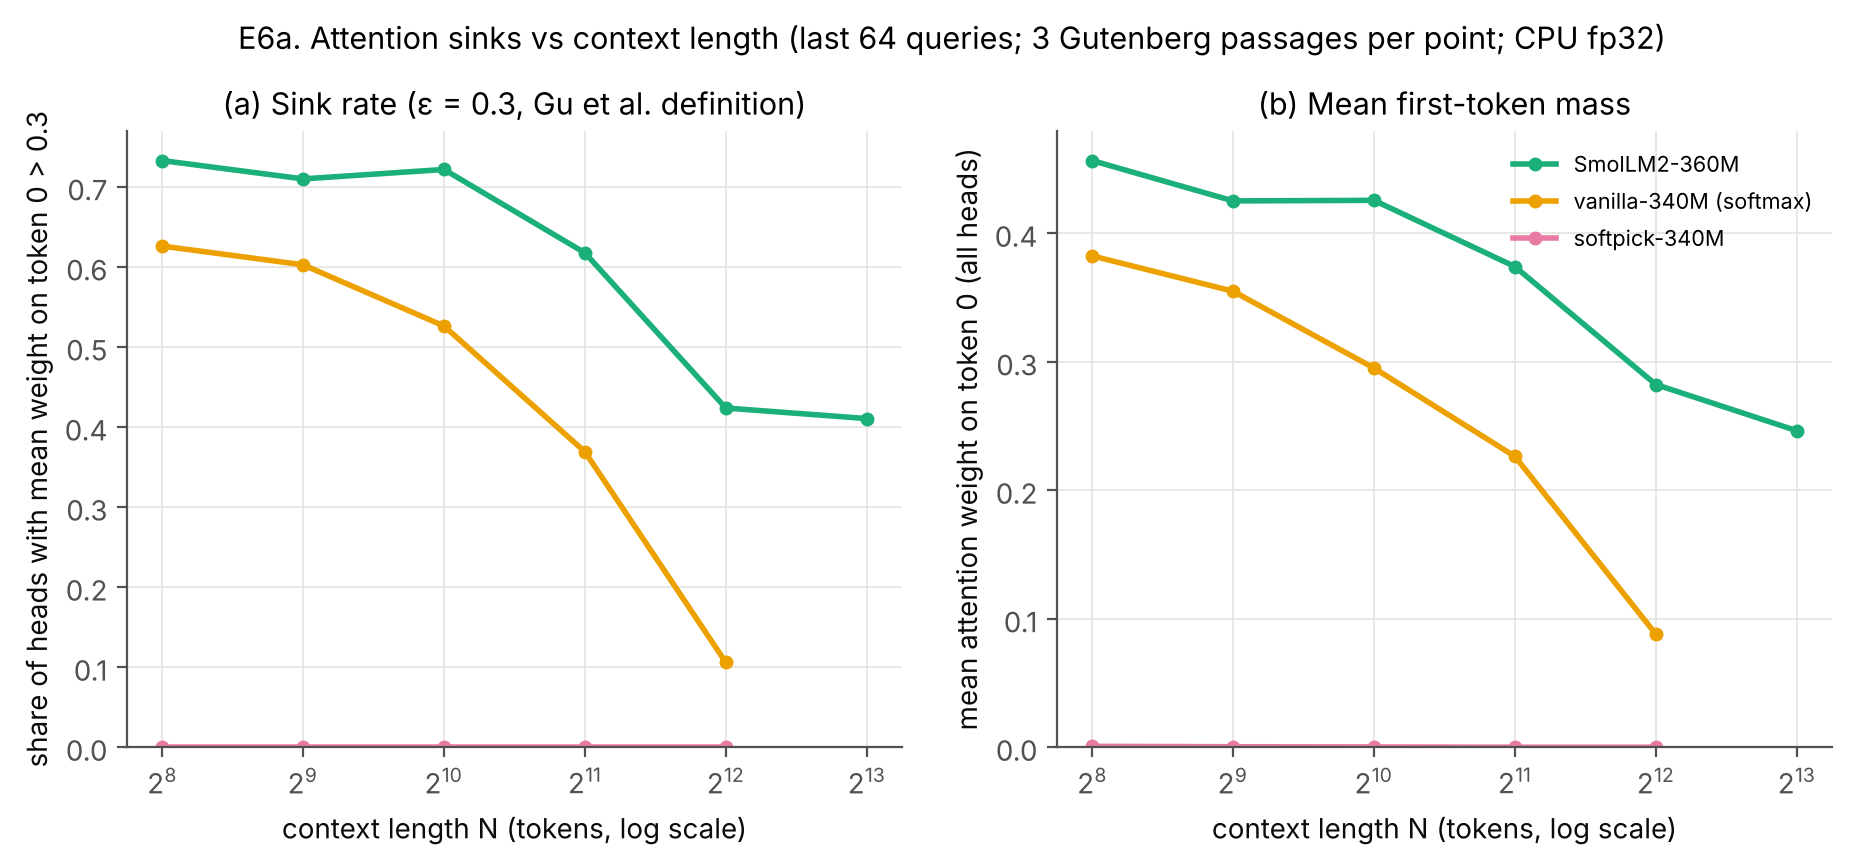
\includegraphics[width=\linewidth]{figures/e6_sinks.png}
\caption{Sink rate and mean first-token mass vs.\ context length.}\label{fig:sinks}
\end{figure}
\begin{figure}[t]
\centering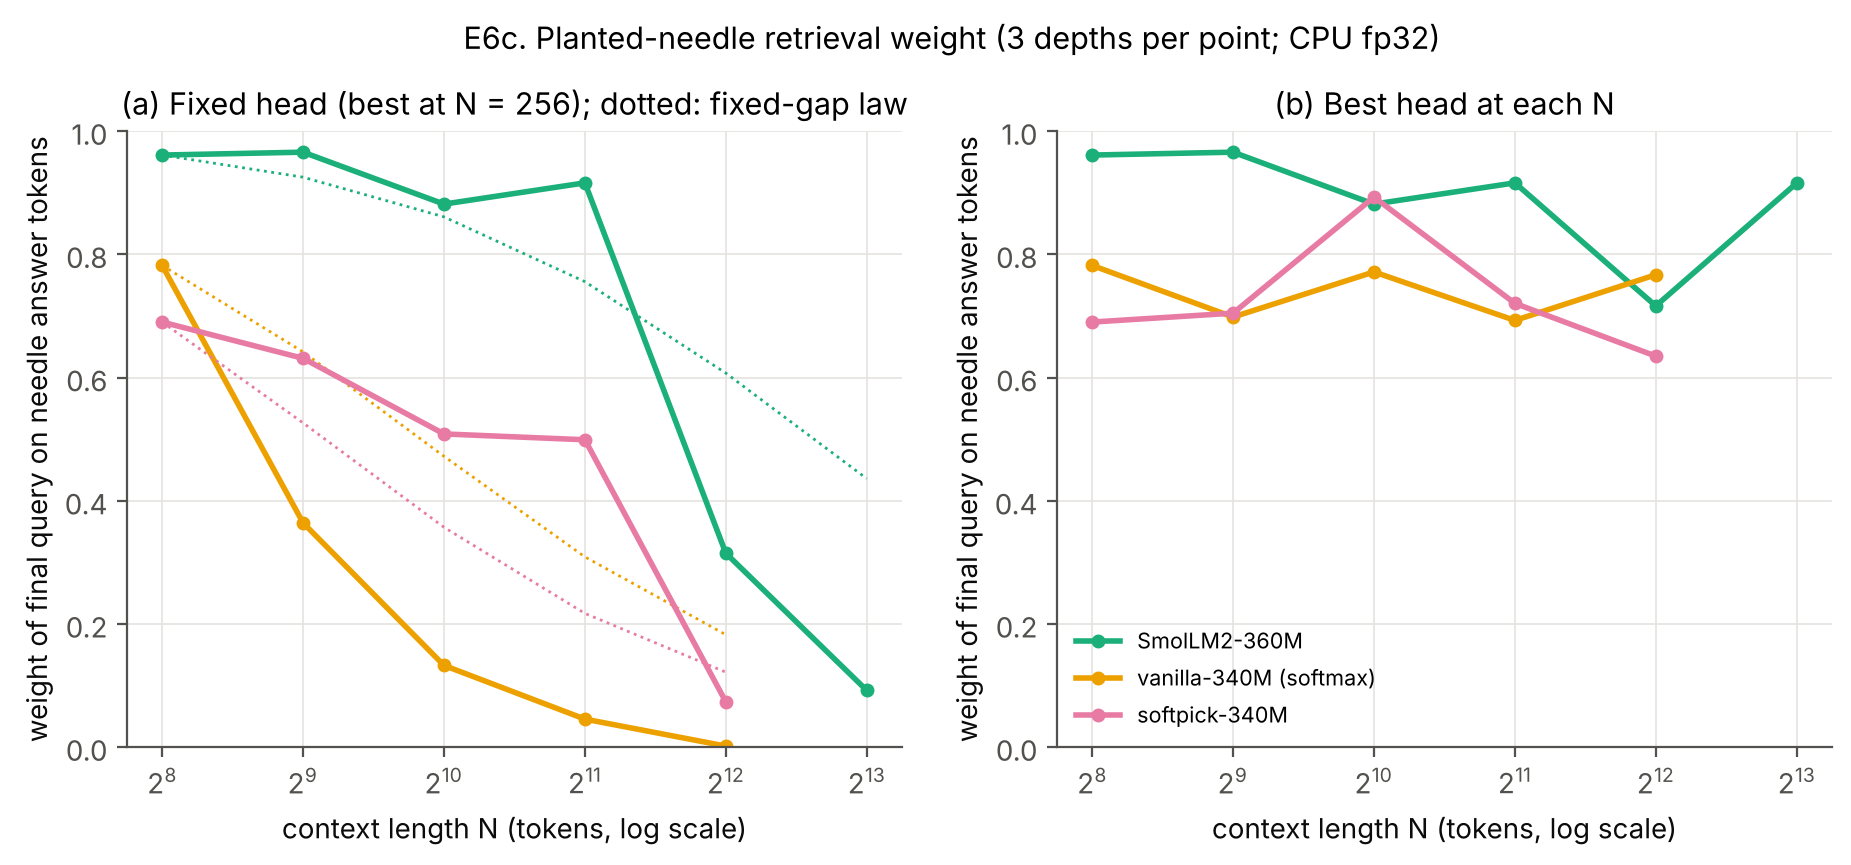
\includegraphics[width=\linewidth]{figures/e6_needle.png}
\caption{Needle weight for a fixed head (dotted: fixed-gap law) and for the best head at each $N$.}\label{fig:needle}
\end{figure}
\paragraph{C2: sinks.} In vanilla-340M, \sinkFirstVanilla\% of heads are sinks at 256 tokens, close to the 63.41\% reported for the authors' 340M softmax model \citep{softpick}. The rate falls to \sinkLastVanilla\% at 4,096 tokens. Gu et al.\ also report their sink metric decreasing with sequence length \citep{gu}. Softpick-340M has no sinks at any length (Table~\ref{tab:e6}, Figure~\ref{fig:sinks}). SmolLM2-360M shows the same decline (Table~\ref{tab:e6}). \pending{Qwen3-0.6B and Gemma-3-1B-it: runs stopped early to save compute; rerun with \texttt{code/e6\_probes.py}.}

\paragraph{C1a: dispersion in real heads.} In vanilla-340M, the best head at 256 tokens falls from weight \needleFixedFirstVanilla{} to \needleFixedLastVanilla{} at 4,096 tokens, faster than the fixed-gap law. Yet the best head at each length keeps \needleBestLastVanilla{}, and the model answers correctly in \needleTopOneVanilla{} cases (Figure~\ref{fig:needle}). A probe that tracks one head would overstate the loss of retrieval ability.

\section{Log-probability precision and serving engines}\label{sec:logprob}
\begin{itemize}[leftmargin=*,itemsep=1pt]
\item \textbf{vLLM} returns \texttt{logits.log\_softmax(dim=-1, dtype=torch.float32)} \citep{vllm}.
\item \textbf{SGLang} casts logits to float32. Greedy requests use \texttt{log\_softmax}, and standard sampling returns \texttt{torch.log(probs)} \citep{sglang}.
\item \textbf{The exception:} with \texttt{--rl-on-policy-target} and deterministic inference, SGLang computes \texttt{log\_softmax} in bfloat16.
\item \textbf{The cost on synthetic logits:} with a 151,936-token vocabulary, bfloat16 \texttt{log\_softmax} returns exactly 0 once the target leads by gap \logpBfGap{} ($p\gtrsim0.996$). fp32 does so only at gap \logpFpGap.
\end{itemize}
\pending{E7: exact-zero rate on real text; B4: returned log-probs from running servers.}

\section{Implications for serving}
\begin{itemize}[leftmargin=*,itemsep=1pt]
\item \textbf{KV eviction.} Window-only eviction fails unless the first tokens are kept \citep{streamingllm}. Our matched pair shows sink mass shrinking with context, and absent under softpick, so the value of pinning the first page may depend on both (inference; tested by B5).
\item \textbf{Log-prob APIs.} Default paths are float32. Users of RL on-policy mode should expect exact zeros on confident tokens (established in code).
\item \textbf{Training numerics.} Collapse thresholds depend on the class count, so the published constants are not safe margins for large vocabularies (established, CPU).
\end{itemize}

\section{Threats to validity}
\begin{itemize}[leftmargin=*,itemsep=1pt]
\item \textbf{Hardware:} CPU kernels only (B6 checks CUDA).
\item \textbf{Scale:} models of 340M--1B parameters at $\leq$8,192 tokens.
\item \textbf{Samples:} three passages and three depths per point, with no confidence intervals in this draft.
\item \textbf{Definitions:} our sink metric averages over the last 64 queries.
\item \textbf{Implementation:} the fixes are our translations of the published code.
\end{itemize}

\section{Artifact availability}\label{sec:artifact}
Code, raw JSON, logs and validation results are in \texttt{reports/softmax\_paper\_v3/} of the author's repository: \texttt{code/}, \texttt{data/}, \texttt{data/validate\_models.json}, and GPU scripts in \texttt{code/gpu/}. B5's success criterion is pre-registered in its docstring. The survey and the census of 36 model families are in the companion report \citep{v2report}.

\bibliography{generated/refs}
\bibliographystyle{tmlr}
\end{document}
